\documentclass{article}
\usepackage[utf8]{inputenc}
\usepackage{tikz}
\usetikzlibrary{shapes.geometric, arrows}
\renewcommand\familydefault{\sfdefault}

\tikzstyle{startstop} = [rectangle, rounded corners, text width=3cm, minimum width=3cm, minimum height=1cm,text centered, draw=black, fill=red!50]

\tikzstyle{io} = [trapezium, trapezium left angle=70, trapezium right angle=110, text width=3cm, minimum width=3cm, minimum height=1cm, text centered, draw=black, fill=blue!50]

\tikzstyle{process} = [rectangle, text width=3cm, minimum width=3cm, minimum height=1cm, text centered, draw=black, fill=orange!70]

\tikzstyle{decision} = [diamond, text width=3cm, minimum width=3cm, minimum height=1cm, text centered, draw=black, fill=green!50]

\tikzstyle{arrow} = [thick,->,>=stealth]

\begin{document}
\pagenumbering{gobble}
\section*{Houdini Event Handling}

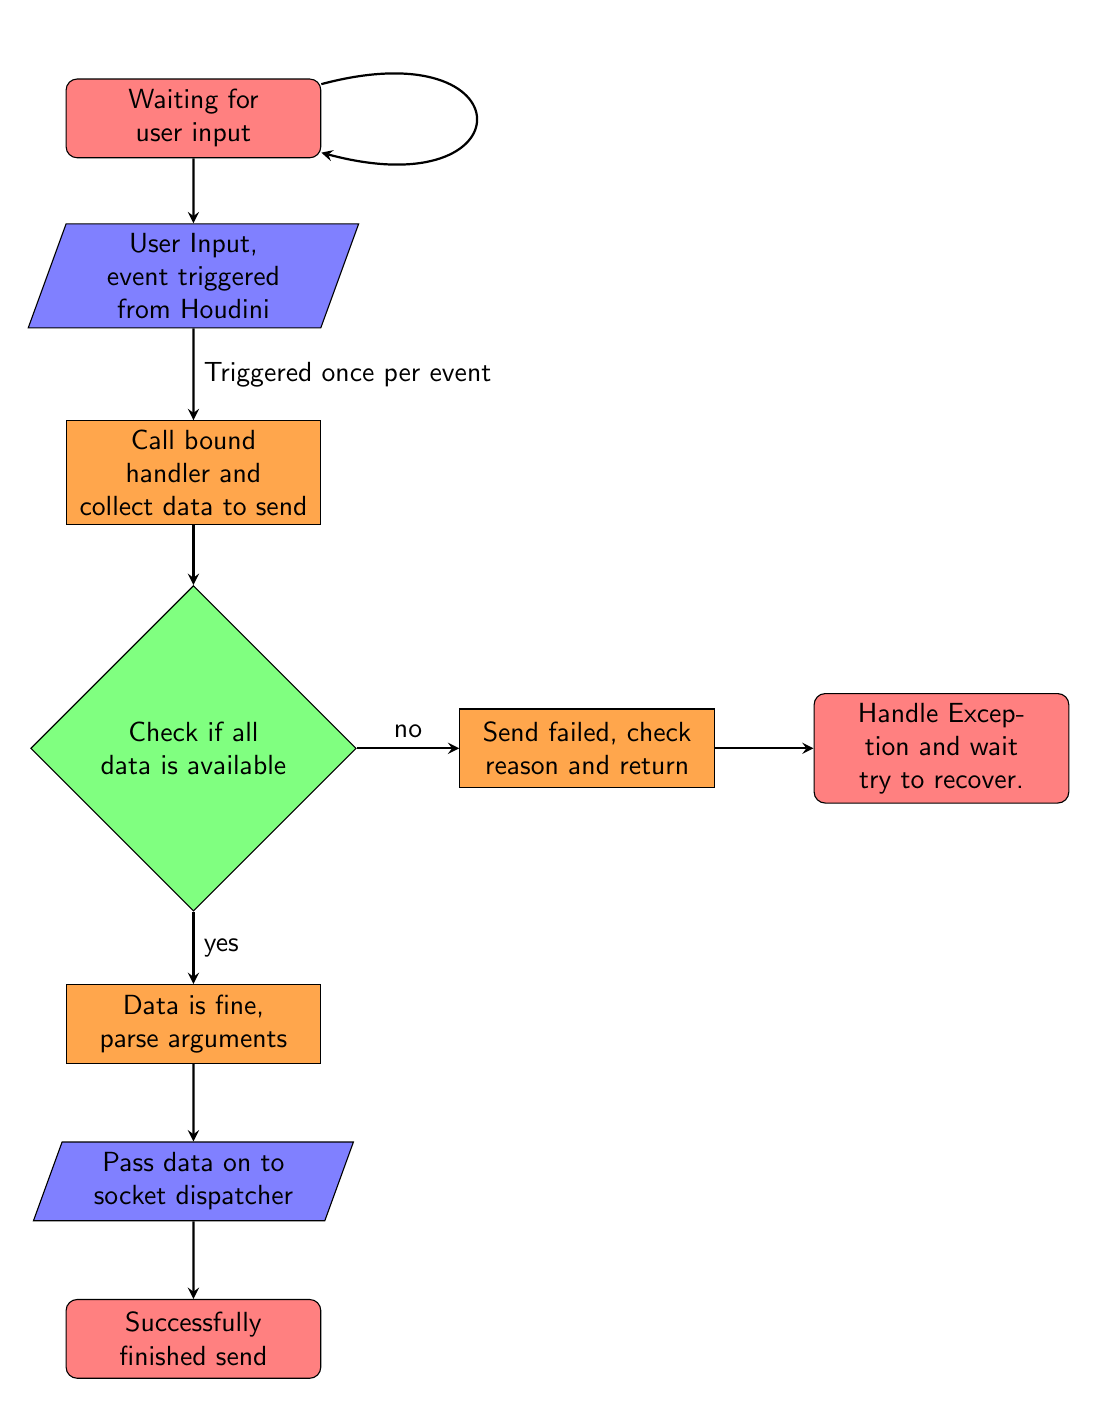
\begin{tikzpicture}[node distance=2cm]

\node (start) [startstop] {Waiting for user input};
\node (input1) [io, below of=start] {User Input, event triggered from Houdini};
\node (process1) [process, yshift=-0.5cm, below of=input1] {Call bound handler and collect data to send};
\node (decision1) [decision, yshift=-1.5cm, below of=process1] {Check if all data is available};
\node (process2a) [process, yshift=-1.5cm, below of=decision1] {Data is fine, parse arguments};
\node (process2b) [process, xshift=3cm, right of=decision1] {Send failed, check reason and return};
\node (endFailed) [startstop, xshift=2.5cm, right of=process2b] {Handle Exception and wait try to recover.};
\node (output) [io, below of=process2a] {Pass data on to socket dispatcher};
\node (end) [startstop, below of=output] {Successfully finished send};

\draw [arrow, loop right] (start) to (start);
\draw [arrow] (start) -- (input1);
\draw [arrow] (input1) -- node [anchor=west] {Triggered once per event} (process1);
\draw [arrow] (process1) -- (decision1);
\draw [arrow] (decision1) -- node [anchor=west] {yes} (process2a);
\draw [arrow] (decision1) -- node [anchor=south] {no} (process2b);
\draw [arrow] (process2b) -- (endFailed);
\draw [arrow] (process2a) -- (output);
\draw [arrow] (output) -- (end);

\end{tikzpicture}

\end{document}